\documentclass[11pt]{article}
\usepackage{graphicx}
\usepackage{float}
\usepackage{hyperref}
\usepackage{natbib}

\setlength{\textwidth}{6.5in}
\setlength{\headheight}{0in}
\setlength{\textheight}{8.0in}
\setlength{\hoffset}{0in}
\setlength{\voffset}{0in}
\setlength{\oddsidemargin}{0in}
\setlength{\evensidemargin}{0in}

\title{Computational Physics PS-1 Report}
  
\author{Tongzhou Wang, GitHub account: TZW56203, repository: phys-ga2000}
\date{September 9, 2024}

\begin{document}

\maketitle

\abstract{This is my report for problem set 1. I briefly wrote about my goals for this course, my background in programming, and my plans for the future. I familiarize myself with \texttt{matplotlib} and \texttt{numpy} in Python to plot a Gaussian with a mean of 0 and a standard deviation of 3.}

\section{Goals, Background, and Plans}
\label{sec:intro}
My goals for this course include learning some computational techniques that will be helpful for research, fulfilling the PhD requirement, and striving to get a good grade.

I have learnt some basic C++ in high school. I have taken a Python programming course in my undergraduate study. In my undergraduate research, I have used Jupyter Notebook for simulation projects.

I want to do a postdoc after obtaining my PhD and find a job in academia. But I can also accept working in industry.

\section{Plotting a Gaussian}
\label{sec:methods}

\begin{figure}[H]
    \centering
    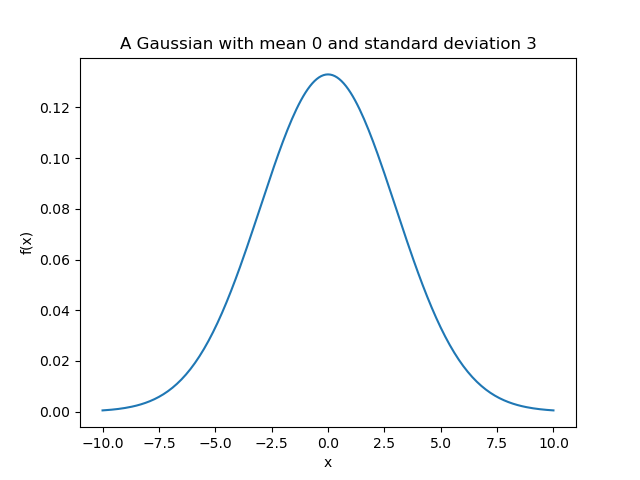
\includegraphics[scale = 1]{images/gaussian.png}
    \caption{A Gaussian with mean 0 and standard deviation 3.}
    \label{fig:gaussian}
\end{figure}

\end{document}

 
 
